\documentclass[tikz,border=10pt]{standalone}
\usepackage[utf8]{vietnam}
\usepackage{tikz}
\usepackage{chemformula} % For chemical equations
\usetikzlibrary{calc, patterns, decorations.pathmorphing, decorations.markings, arrows.meta, shapes.geometric}

\begin{document}
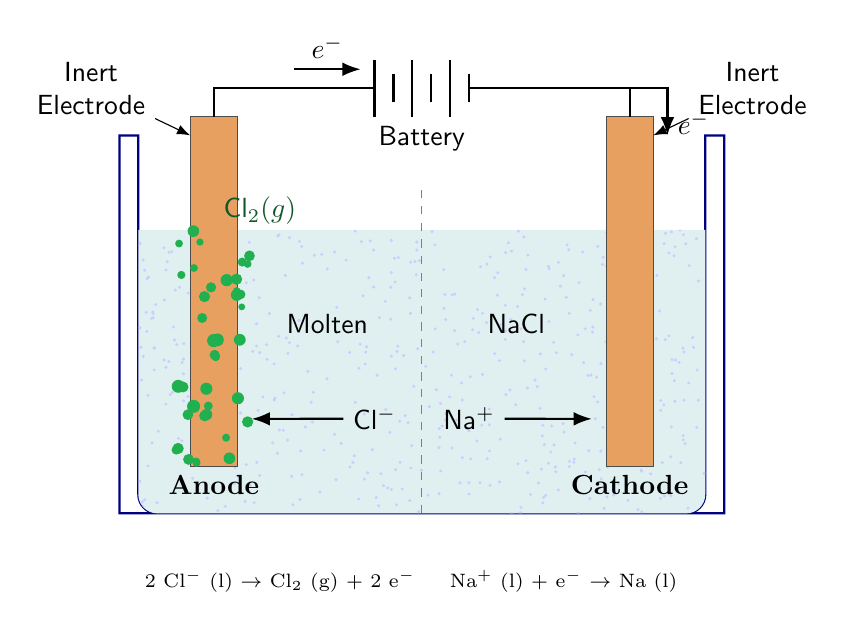
\begin{tikzpicture}[
    font=\sffamily,
    >=Latex,
    scale=1.2
]

    % Parameters
    \def\cupWidth{6}
    \def\cupHeight{4}
    \def\liquidHeight{3}
    \def\electrodeWidth{0.5}
    \def\electrodeHeight{3.5}
    \def\wireHeight{4.5}

    % Define colors
    \definecolor{liquidColor}{HTML}{E0F0F0}
    \definecolor{electrodeColor}{HTML}{E8A060}
    \definecolor{bubbleColor}{HTML}{20B050} % Greenish for Cl2

    % 1. Beaker/Container
    \draw[thick, blue!50!black, fill=white] (-0.2, 0) -- (-0.2, \cupHeight) -- (0, \cupHeight) -- (0, 0.2) arc(180:270:0.2) -- (\cupWidth-0.2, 0) arc(270:360:0.2) -- (\cupWidth, \cupHeight) -- (\cupWidth+0.2, \cupHeight) -- (\cupWidth+0.2, 0) -- cycle;
    
    % Liquid
    \fill[liquidColor] (0, 0.2) arc(180:270:0.2) -- (\cupWidth-0.2, 0) arc(270:360:0.2) -- (\cupWidth, \liquidHeight) -- (0, \liquidHeight) -- cycle;
    
    % Liquid Pattern (Stippling/Dots) - using random dots for effect
    \begin{scope}
        \clip (0, 0.2) arc(180:270:0.2) -- (\cupWidth-0.2, 0) arc(270:360:0.2) -- (\cupWidth, \liquidHeight) -- (0, \liquidHeight) -- cycle;
        \foreach \i in {1,...,500} {
            \fill[blue!20] ({rnd*\cupWidth}, {rnd*\liquidHeight}) circle (0.5pt);
        }
    \end{scope}

    % Dashed line in middle
    \draw[dashed, black!50] (\cupWidth/2, 0) -- (\cupWidth/2, \liquidHeight + 0.5);

    % 2. Electrodes
    % Anode (Left)
    \coordinate (AnodeCenter) at (0.8, \liquidHeight - \electrodeHeight/2 + 0.5);
    \filldraw[fill=electrodeColor, draw=black!70] (0.55, 0.5) rectangle (1.05, \cupHeight+0.2);
    
    % Cathode (Right)
    \filldraw[fill=electrodeColor, draw=black!70] (\cupWidth-1.05, 0.5) rectangle (\cupWidth-0.55, \cupHeight+0.2);

    % 3. Bubbles at Anode (Cl2)
    \foreach \i in {1,...,40} {
        \fill[bubbleColor] (0.4 + rnd*0.8, 0.5 + rnd*2.5) circle ({1pt + rnd*1pt});
    }
    \node[anchor=west, bubbleColor!50!black] at (0.8, 3.2) {Cl$_2(g)$};

    % 4. Wiring and Battery
    % Wire Anode -> Battery
    \draw[thick] (0.8, \cupHeight+0.2) -- (0.8, \wireHeight) -- (\cupWidth/2 - 0.5, \wireHeight);
    
    % Wire Cathode -> Battery
    \draw[thick] (\cupWidth-0.8, \cupHeight+0.2) -- (\cupWidth-0.8, \wireHeight) -- (\cupWidth/2 + 0.5, \wireHeight);

    % Battery Symbol
    \draw[thick] (\cupWidth/2 - 0.5, \wireHeight - 0.3) -- (\cupWidth/2 - 0.5, \wireHeight + 0.3); % Long
    \draw[thick] (\cupWidth/2 - 0.3, \wireHeight - 0.15) -- (\cupWidth/2 - 0.3, \wireHeight + 0.15); % Short
    \draw[thick] (\cupWidth/2 - 0.1, \wireHeight - 0.3) -- (\cupWidth/2 - 0.1, \wireHeight + 0.3); % Long
    \draw[thick] (\cupWidth/2 + 0.1, \wireHeight - 0.15) -- (\cupWidth/2 + 0.1, \wireHeight + 0.15); % Short
    \draw[thick] (\cupWidth/2 + 0.3, \wireHeight - 0.3) -- (\cupWidth/2 + 0.3, \wireHeight + 0.3); % Long
    \draw[thick] (\cupWidth/2 + 0.5, \wireHeight - 0.15) -- (\cupWidth/2 + 0.5, \wireHeight + 0.15); % Short
    
    \node[below] at (\cupWidth/2, \wireHeight - 0.3) {Battery};

    % Electron Flow decoration
    \draw[->, thick, shorten >= 5pt, shorten <= 5pt] (1.5, \wireHeight + 0.2) -- (2.5, \wireHeight + 0.2) node[midway, above] {$e^-$};
    \draw[->, thick] (\cupWidth-0.8, \wireHeight) -- (\cupWidth-0.4, \wireHeight) -- (\cupWidth-0.4, \wireHeight-0.5) node[right, near end] {$e^-$};


    % 5. Labels and Ions
    % Text "Inert Electrode"
    \node[align=center] (InertL) at (-0.5, \wireHeight) {Inert\\Electrode};
    \draw[->] (InertL) -- (0.55, \cupHeight);
    
    \node[align=center] (InertR) at (\cupWidth+0.5, \wireHeight) {Inert\\Electrode};
    \draw[->] (InertR) -- (\cupWidth-0.55, \cupHeight);

    % Molten NaCl
    \node at (\cupWidth/2 - 1, 2) {Molten};
    \node at (\cupWidth/2 + 1, 2) {NaCl};

    % Ions
    \node (ClIon) at (\cupWidth/2 - 0.5, 1) {Cl$^-$};
    \draw[->, thick] (ClIon) -- (1.2, 1);
    
    \node (NaIon) at (\cupWidth/2 + 0.5, 1) {Na$^+$};
    \draw[->, thick] (NaIon) -- (\cupWidth-1.2, 1);

    % Anode / Cathode
    \node[font=\bfseries] at (0.8, 0.3) {Anode};
    \node[font=\bfseries] at (\cupWidth-0.8, 0.3) {Cathode};

    % 6. Equations
    \node[below, align=left,font=\scriptsize] at (1.5, -0.5) {2 Cl$^-$ (l) $\rightarrow$ Cl$_2$ (g) + 2 e$^-$};
    \node[below, align=left,font=\scriptsize] at (\cupWidth-1.5, -0.5) {Na$^+$ (l) + e$^-$ $\rightarrow$ Na (l)};

\end{tikzpicture}
\end{document}
